%! TEX program = xelatex
\PassOptionsToPackage{unicode}{hyperref}
% \documentclass[draft]{beamer}
\documentclass{beamer}

\usepackage{kotex}
\usepackage{minted}

\vfuzz=30pt
\hfuzz=5pt

%%%%%%%%%%%%%%%%%%%%%
%  Beamer Settings  %
%%%%%%%%%%%%%%%%%%%%%
\usetheme[numbering=fraction]{metropolis}
\usecolortheme{rose}
\useoutertheme[subsection=false]{miniframes}

\setbeamertemplate{itemize item}[square]
\setbeamertemplate{itemize subitem}[triangle]
\setbeamertemplate{itemize subsubitem}[circle]


%%%%%%%%%%%%%%%%%%%
%  Font Settings  %
%%%%%%%%%%%%%%%%%%%
\usepackage[factor=500]{microtype}

\usefonttheme{professionalfonts} % required for mathspec
\usepackage{mathspec}

\setmathsfont(Digits)[%
  Numbers={Lining, Proportional}
]{Fira Sans}
\setsansfont[%
  BoldFont={Fira Sans SemiBold},
  Numbers={OldStyle}
]{Fira Sans}
\setsanshangulfont{Noto Sans CJK KR}[%
  AutoFakeSlant=0.18,
  FontFace={m}{up}{Font=*}
]

\newfontfamily\NotoSansMonoExtraCondensed{Noto Sans Mono ExtraCondensed}
\RenewDocumentCommand\UrlFont{}{\NotoSansMonoExtraCondensed}
\NewDocumentCommand\textct{m}{{\NotoSansMonoExtraCondensed#1}}

%%%%%%%%%%%%%%%%%%%%%
%  Minted Settings  %
%%%%%%%%%%%%%%%%%%%%%
\renewcommand\theFancyVerbLine{\textsf{\tiny\arabic{FancyVerbLine}}}
%
\newminted{shell}{
  escapeinside=||,
  autogobble,
  breaklines,
  frame=single,
  fontsize=\footnotesize}
\newminted{vim}{
  escapeinside=||,
  autogobble,
  linenos,
  breaklines,
  numbersep=5pt,
  frame=single,
  fontsize=\footnotesize}

%%%%%%%%%%%%%%%%%%%%%%%
% Custom Settings  %
%%%%%%%%%%%%%%%%%%%%%%%
\NewDocumentCommand\tpc{}{\textperiodcentered}
\NewDocumentCommand\tat{}{\textasciitilde}
\NewDocumentCommand\tla{}{\textleftarrow}
\NewDocumentCommand\tra{}{\textrightarrow}
\NewDocumentCommand\tua{}{\textuparrow}
\NewDocumentCommand\tda{}{\textdownarrow}
\NewDocumentCommand\tbs{}{\textbackslash}
\NewDocumentCommand\vpad{}{\vspace{1em}}

%%%%%%%%%%%%%%%%%%%%%%%
%  Document Settings  %
%%%%%%%%%%%%%%%%%%%%%%%
\title{\TeX{}nical Vim}
\author{이재호}
\institute{서울대학교 전기\tpc{}정보공학부/KTUG}
\date{2020년 2월 15일}

%%%%%%%%%%%%%%
%  Document  %
%%%%%%%%%%%%%%
\begin{document}
% \RenewDocumentCommand\pause{o}{}

\maketitle

%%%%% Hook %%%%%
\begin{frame}[plain]{}
  \begin{tabular}{cccc}
    
\includegraphics[width=0.21\linewidth]{figures/logo-atom} &
    
\includegraphics[width=0.21\linewidth]{figures/logo-bbedit} &
    
\includegraphics[width=0.21\linewidth]{figures/logo-eclipse} &
    
\includegraphics[width=0.21\linewidth]{figures/logo-emacs} \\
    
\includegraphics[width=0.21\linewidth]{figures/logo-gedit} &
    
\includegraphics[width=0.21\linewidth]{figures/logo-notepad} &
    
\includegraphics[width=0.21\linewidth]{figures/logo-notepad++} &
    
\includegraphics[width=0.21\linewidth]{figures/logo-sublime-text-3} \\
    
\includegraphics[width=0.21\linewidth]{figures/logo-texshop} &
    
\includegraphics[width=0.21\linewidth]{figures/logo-texworks} &
    
\includegraphics[width=0.21\linewidth]{figures/logo-vim} &
    
\includegraphics[width=0.21\linewidth]{figures/logo-vscode}
  \end{tabular}
\end{frame}

\begin{frame}[plain]{Editor War (1985\tat{}현재)}
  \centering
\includegraphics[width=0.8\linewidth]{figures/emacs-vs-vim}
\end{frame}

\begin{frame}[plain]{}
  \Large\centering
  그렇다면 어떤 에디터를 쓰는게 제일 좋을까요?\\\pause\vpad
  \large
  여러분의 취향에 맞는 에디터를 쓰세요!\\\pause\vpad
  \alert{한 가지 취향}과 \alert{가능성}을 소개해드리려고 합니다.
\end{frame}

\begin{frame}[plain]{}
  Vim의 가장 큰 무기는 \alert{원하는대로 만들 수 있다는 것}입니다.\\\pause\vpad
  \begin{columns}
    \begin{column}{0.5\linewidth}
      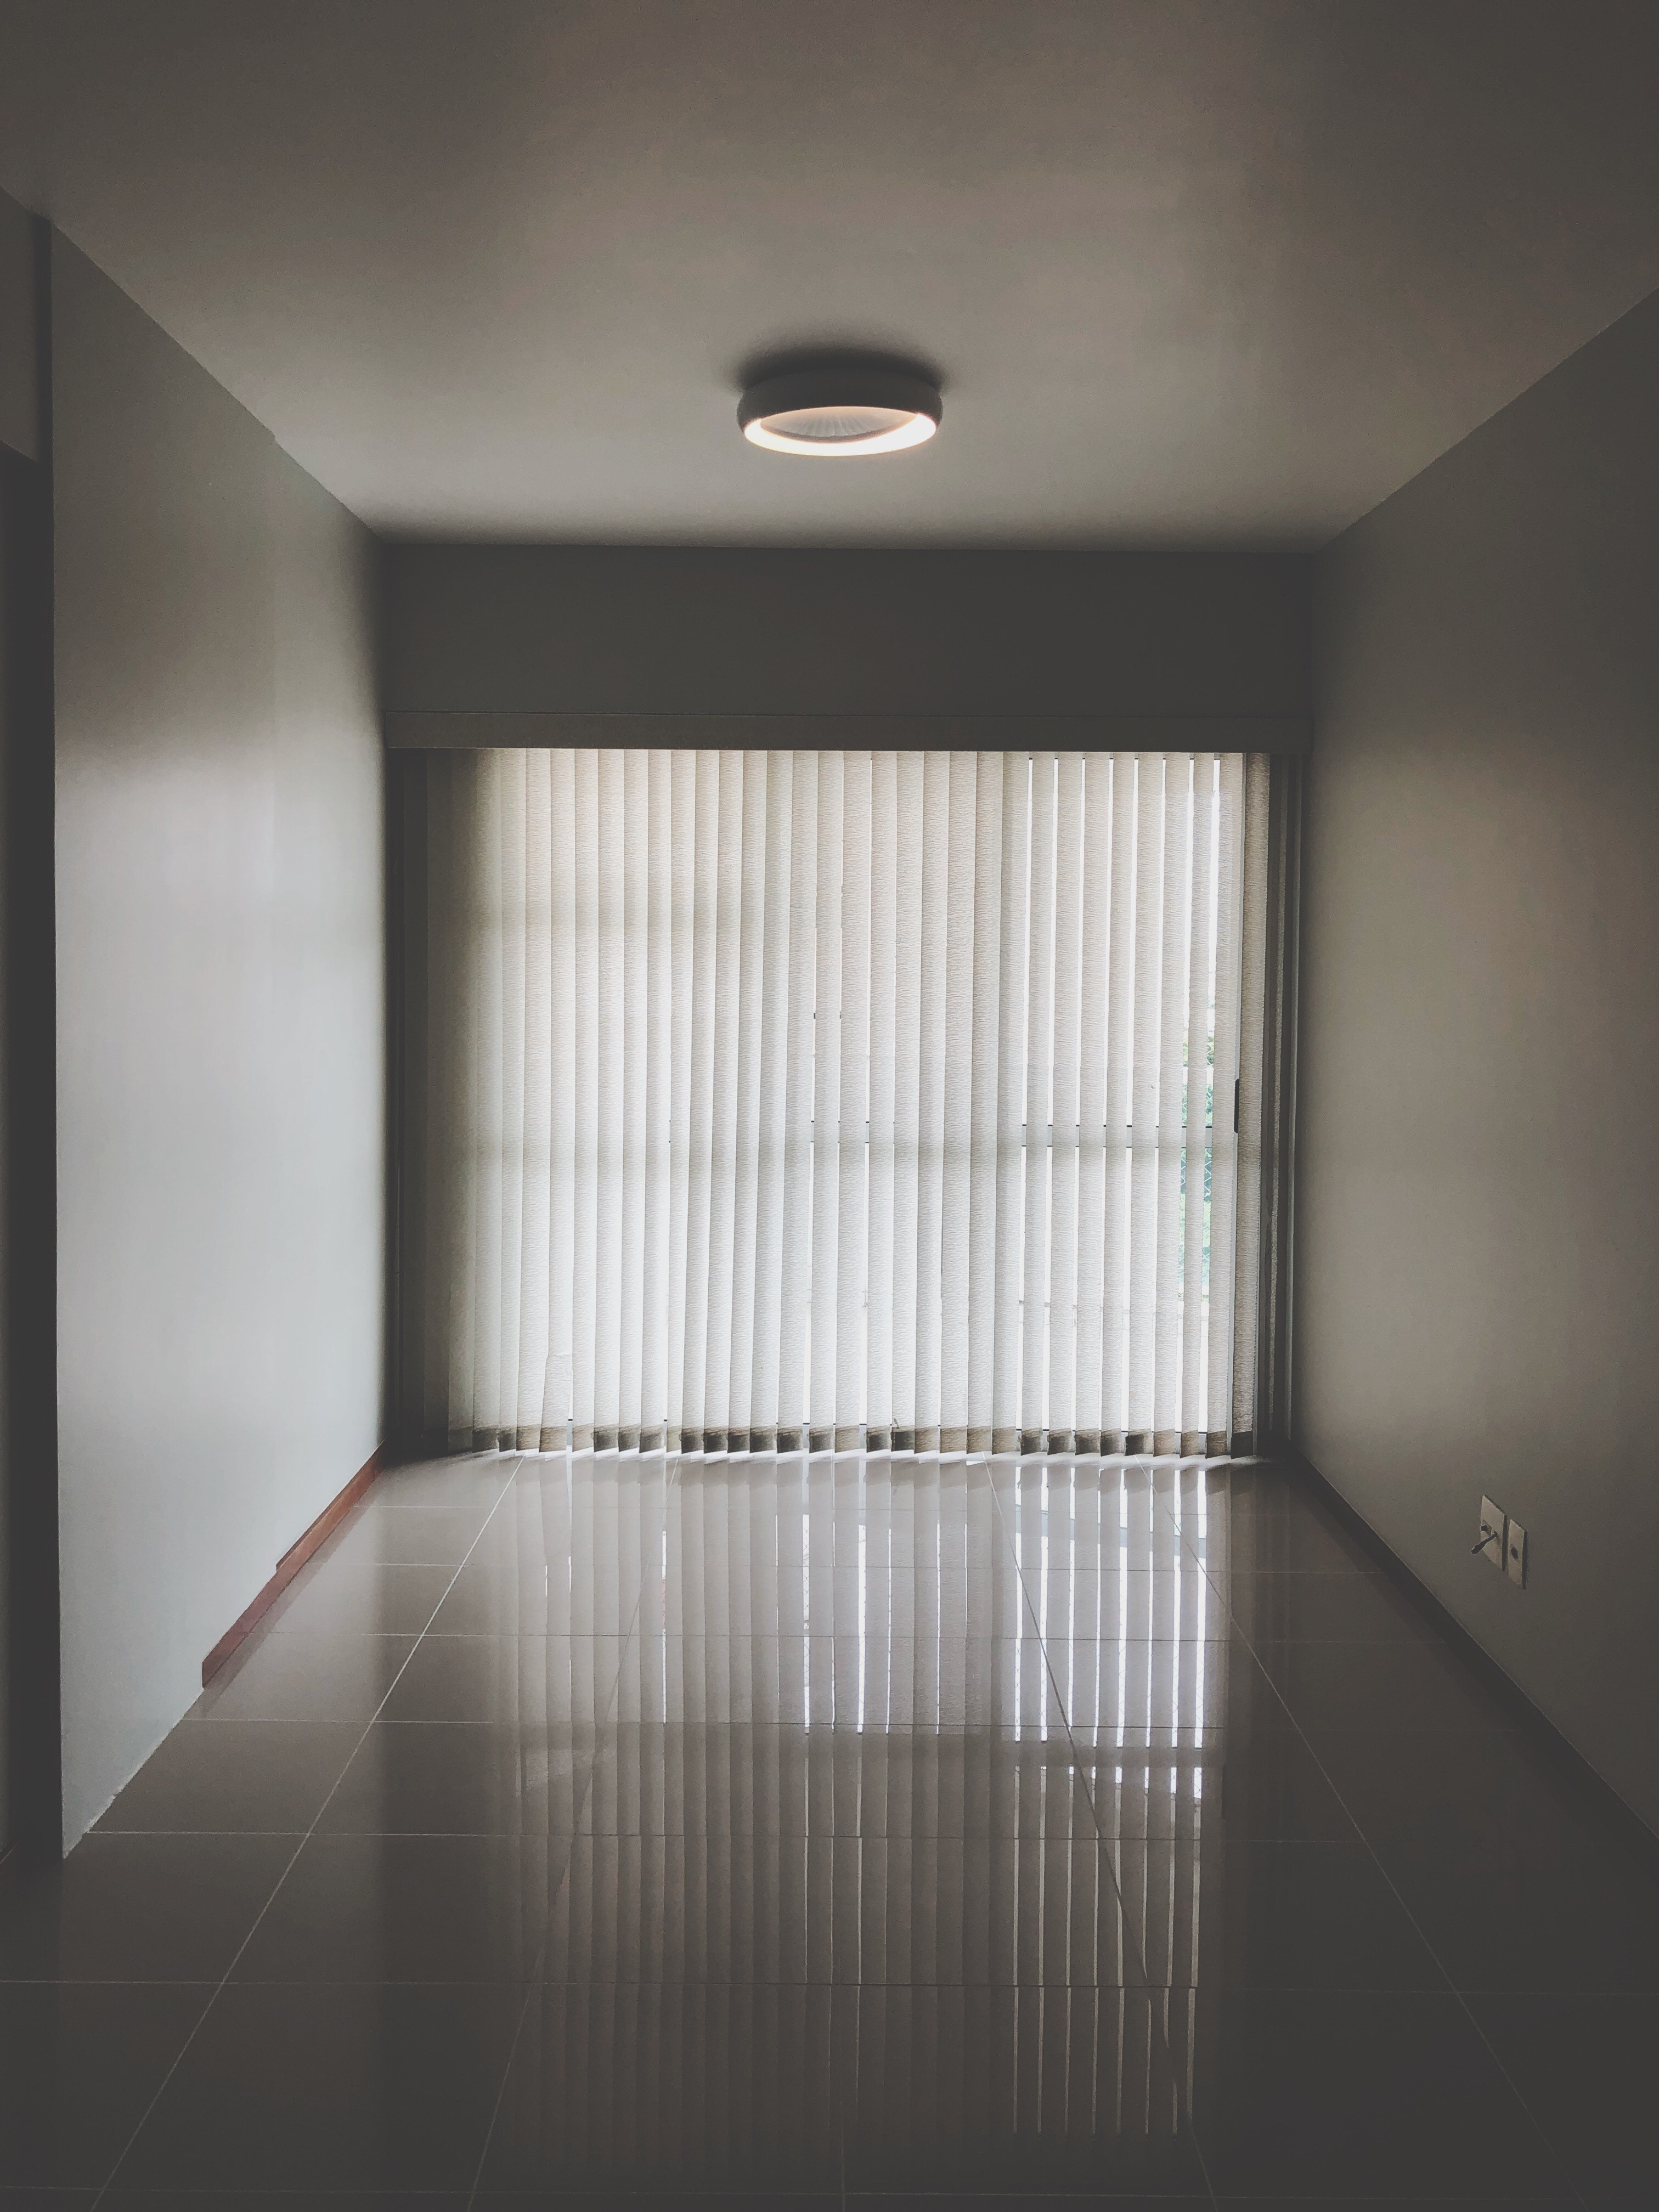
\includegraphics[width=\linewidth]{figures/empty-room}
    \end{column}
    \pause
    \begin{column}{0.5\linewidth}
      \centering
      그러나, 이는 동시에 진입장벽이기도 합니다.\\\pause
      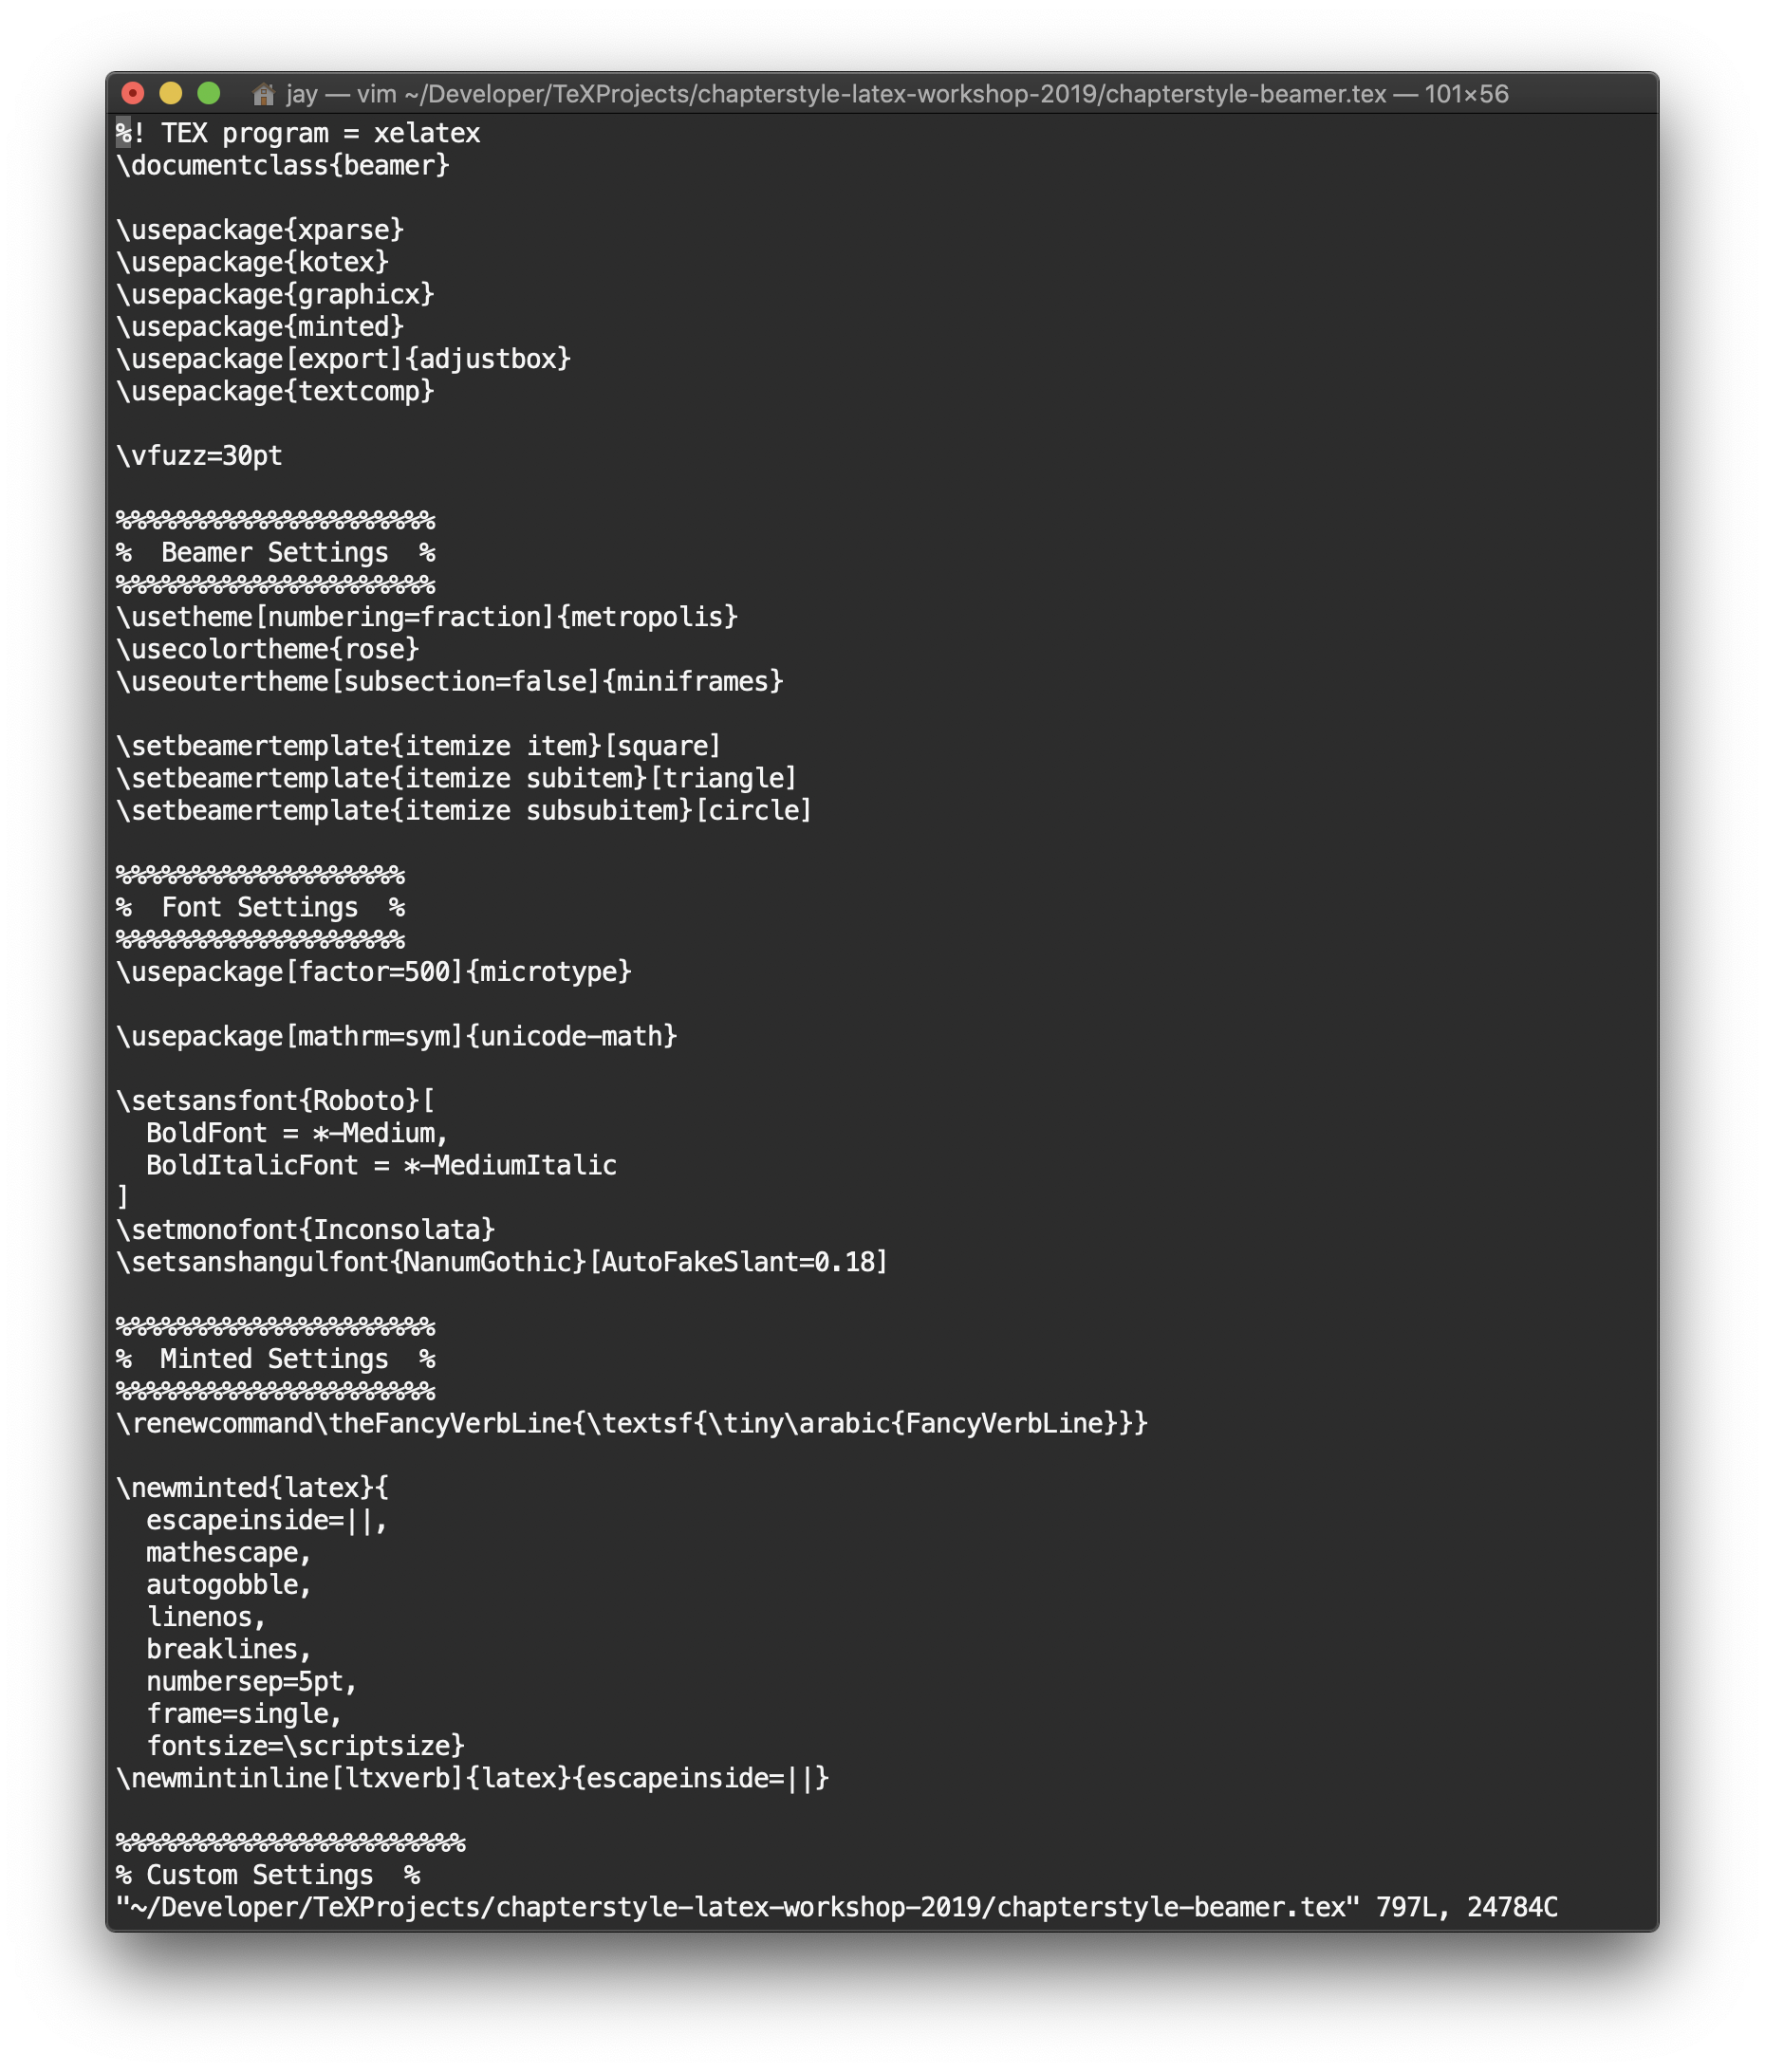
\includegraphics[width=\linewidth]{figures/vanilla-vim}
    \end{column}
  \end{columns}
\end{frame}

\begin{frame}[plain]{가능성}
  \centering\includegraphics[width=\linewidth]{figures/possibility}
\end{frame}

\begin{frame}{본 발표는...}
  \TeX{} 사용자 중
  \begin{enumerate}
    \item Vim에 대해서 들어봤지만 시도하기가 막막하셨던 분들,\pause
    \item Vim을 쓸 줄 알지만 자료가 별로 없어서 \TeX을 Vim에서 쓰지 않았던
      분들,\pause
    \item Vim(혹은 Emacs+AUC\TeX)으로 \TeX을 쓰지만 다른 사람들의 작업 환경이
      궁금하신 분들\pause
  \end{enumerate}
  \vpad
  \centering\alert{Vim으로 \TeX{} 문서를 작성하고 편집하는 효율적인 세팅!}
\end{frame}

\begin{frame}[plain]{}
  \centering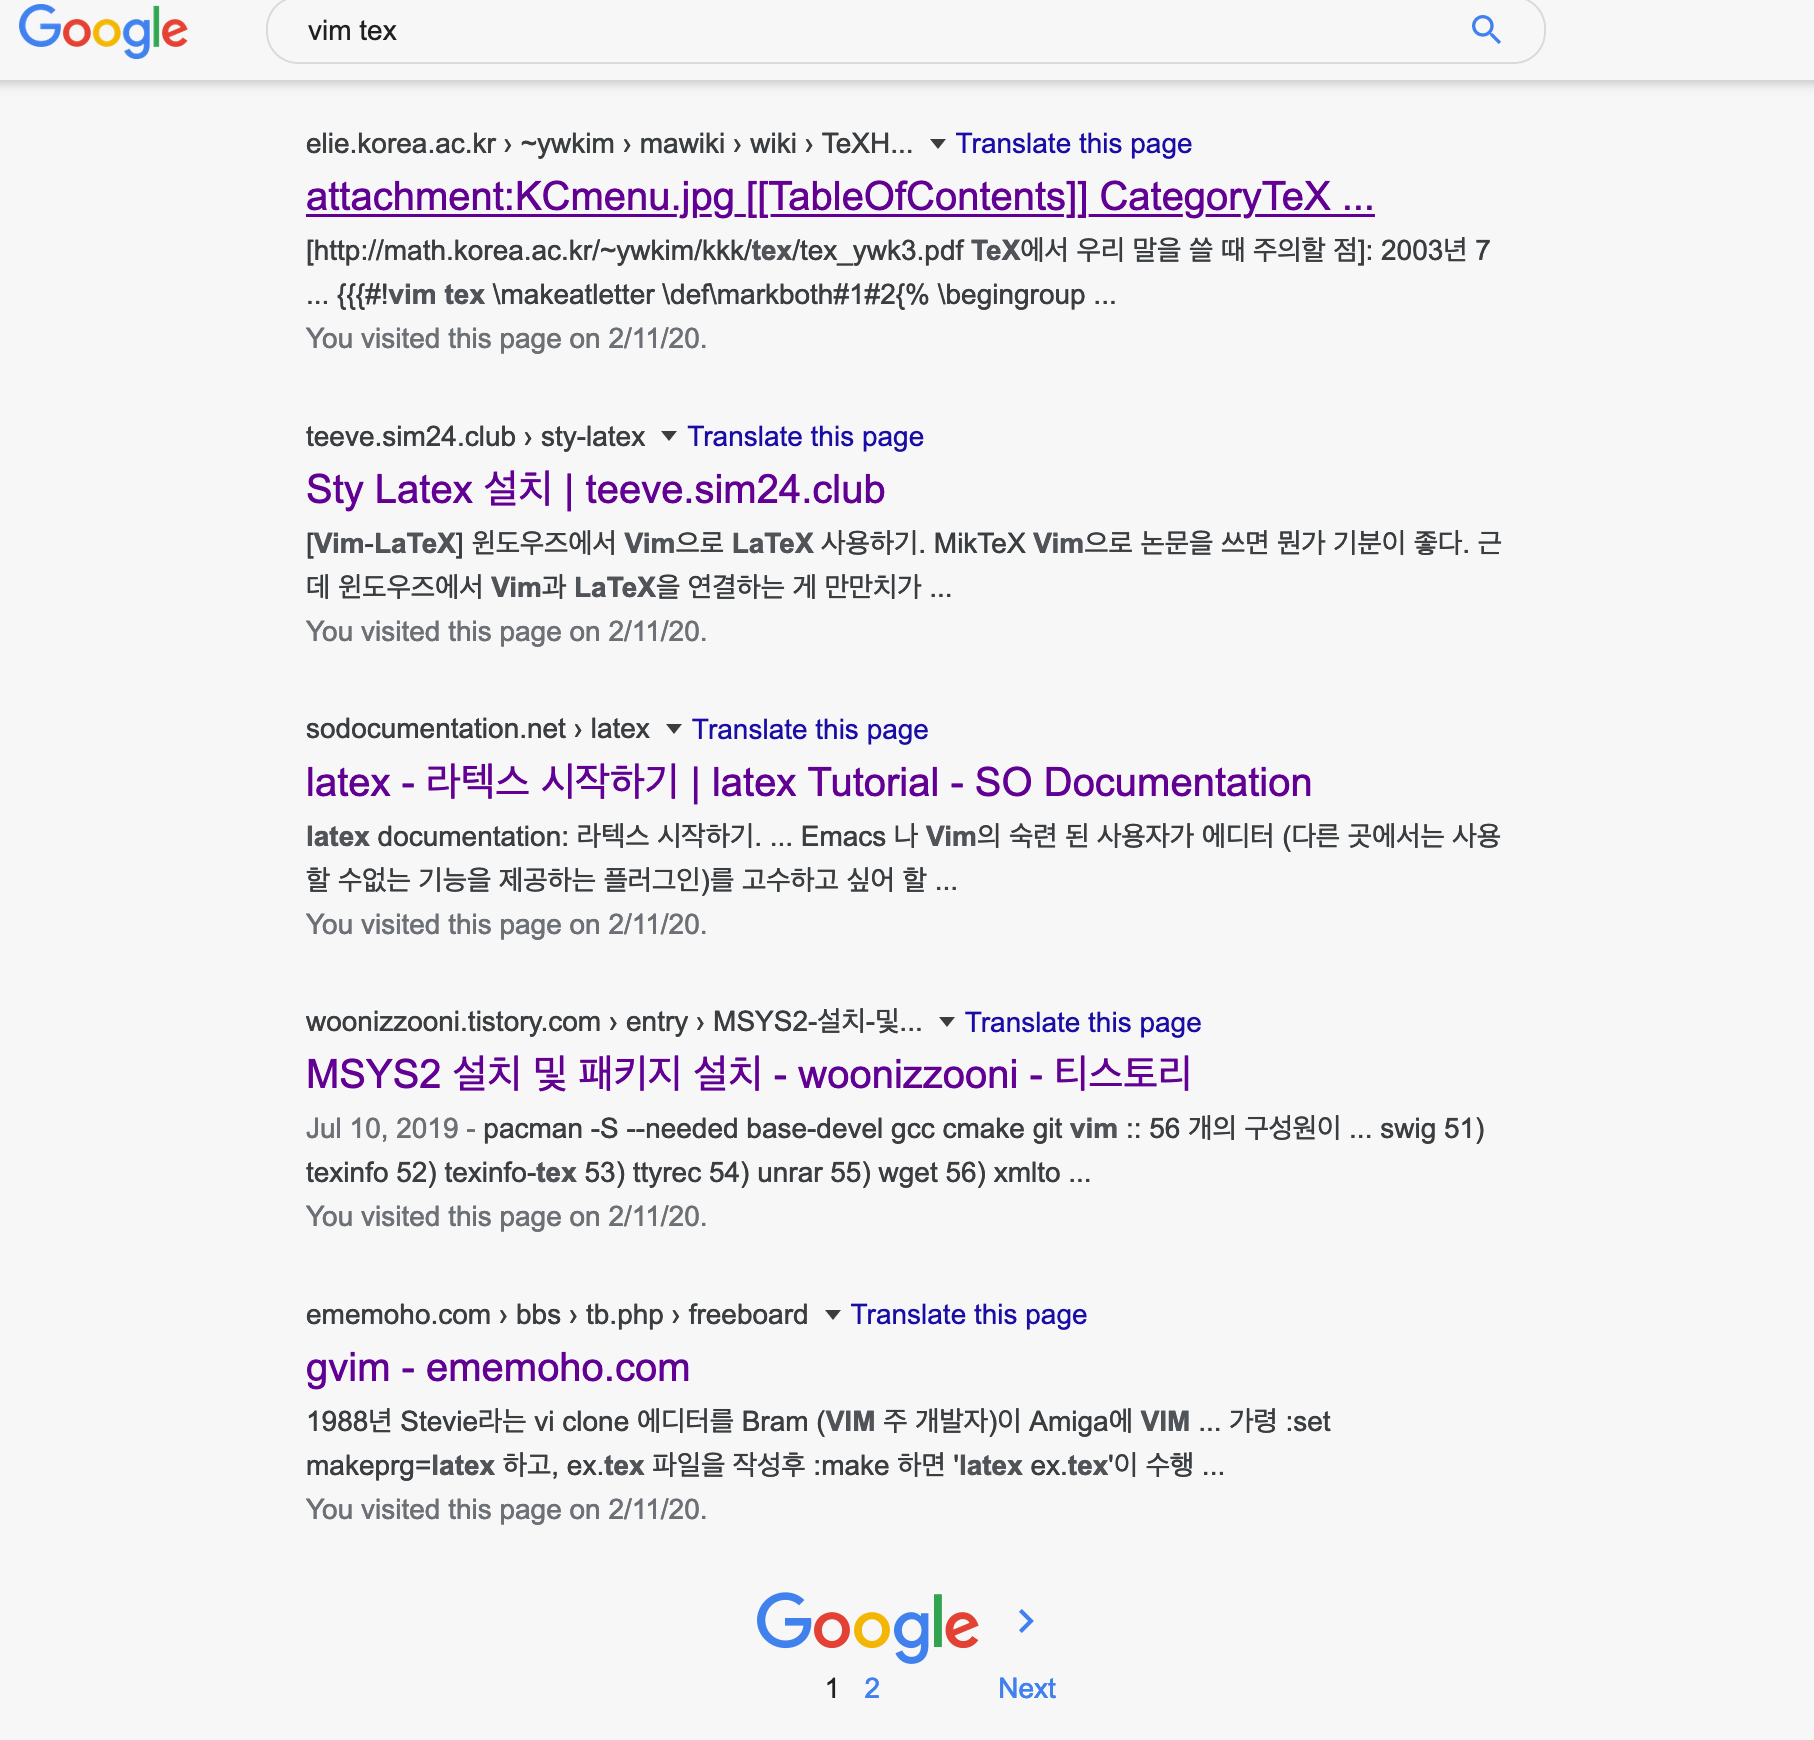
\includegraphics[width=0.8\linewidth]{figures/google-vim-tex-result}
\end{frame}

\frame[plain]{\tableofcontents}

\section{Why Vim?}

\begin{frame}{첫 번째 관문}
  \TeX{}을 처음 깔았을 때 누구나 마주하는 문제:\\\pause\vpad
  \begin{center}\emph{\TeX{} 문서를 어떤 도구로 만들까?}\end{center}
  \pause\vpad

  가장 기본적인 선택지:
  \begin{itemize}
    \item \TeX{}works (Windows)
    \item \TeX{}Shop (macOS)
  \end{itemize}
\end{frame}

\begin{frame}{Vim이 뭔가요?}
  \pause\centering\alert{\Large Vim은 modal(모달) 에디터입니다.}\pause\vpad
  \begin{itemize}
    \item Normal, Insert, Visual, Command-line 모드
      \begin{itemize}
        \item \textcolor{gray}{와 Ex, Select 모드}
      \end{itemize}
    \pause
    \item \alert{Edit}or라는 이름에 걸맞게, 편집하는 일에 특화
      \begin{itemize}
        \item 반복 작업 및 영역 편집
      \end{itemize}
    \pause
    \item 기본적으로는 터미널에서 사용
      \begin{itemize}
        \item 손은 키보드 위에서만
      \end{itemize}
    \pause
    \item \alert{매우 유연한 설정}
      \begin{itemize}
        \item 그만큼 초기 설정은 매우 적음
      \end{itemize}
  \end{itemize}
\end{frame}

\begin{frame}{왜 X 대신 Vim인가요?}
  \begin{itemize}
    \item X = Electron 계열의 에디터 (Atom, Visual Studio Code)\pause
      \begin{itemize}
        \item 장점
          \begin{itemize}
            \item GUI로 동작하므로 진입장벽이 낮음\pause
            \item \alert{Language server}를 통한 강력한 문법 강조 및 자동
              완성\pause
          \end{itemize}
        \item 단점
          \begin{itemize}
            \item (텍스트 편집을 위해서!) 웹 브라우저(Chromium)의 부하\pause
            \item \alert{Language Server Protocol (LSP)}의 등장\pause
          \end{itemize}
      \end{itemize}
    \item X = Emacs\pause
      \begin{itemize}
        \item 장점
          \begin{itemize}
            \item TUI로 동작함\pause
            \item More than an editor\pause
          \end{itemize}
        \item 단점\pause
          \begin{itemize}
            \item TUI로 동작함
            \item More than an editor
          \end{itemize}
      \end{itemize}
  \end{itemize}
\end{frame}

\begin{frame}{2020년의 Vim}
  \begin{itemize}
    \item User Friendly!\pause
      \begin{itemize}
        \item LSP의 혜택으로 강력한 \alert{문법 강조}, \alert{자동 완성},
          \alert{문법 검증}\pause
          \begin{itemize}
            \item LSP가 너무 무겁다면, 기존 방식의 문법팩 사용 가능
          \end{itemize}
        \item 모든 것이 사용자화 가능\pause
        \item 직관적이고 편한 명령어 (동사 + 명사)\pause
        \item 40년이 넘는 자료와 사용자 그룹\pause
        \item 한 가지 일을 하고, 그것을 잘함
          (\href{https://en.wikipedia.org/wiki/Unix_philosophy}{UNIX Philosophy: Do One Thing and Do It Well})\pause
      \end{itemize}
    \item Developer Friendly!\pause
      \begin{itemize}
        \item Lua를 내장한 Neovim의 등장으로 Lua로 스크립팅이 가능해짐
          \textcolor{gray}{(Lua\TeX?)}\pause
        \item 커뮤니티 기반 (무엇이 Vim이고 Neovim일까요?)\\
          \vspace{5pt}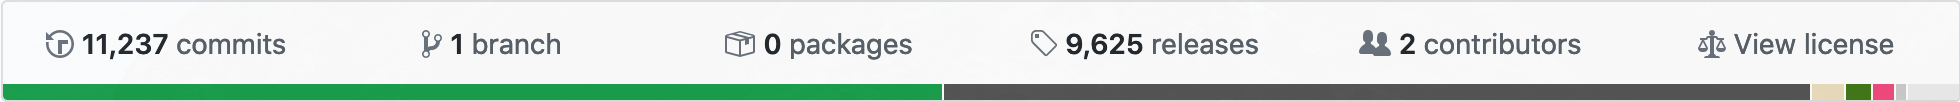
\includegraphics[width=\linewidth]{figures/guess-what-1}\\
          \vspace{2pt}
\includegraphics[width=\linewidth]{figures/guess-what-2}
      \end{itemize}
  \end{itemize}
\end{frame}

\begin{frame}
  
\includegraphics[width=\linewidth]{figures/logo-neovim}
\end{frame}

\section{Vim Setup}

% macOS setup
\begin{frame}[fragile,allowframebreaks]{\TeX{}nical Vim 설정 (for macOS)}
  macOS용 package manager인 \href{https://brew.sh/}{Homebrew}를 사용합니다.
  \begin{enumerate}
    \item \url{https://brew.sh/}를 참고하여 \href{https://brew.sh/}{Homebrew}를 설치합니다.
    \item \href{https://iterm2.com/}{iTerm2},
      \href{https://www.tug.org/mactex/}{Mac\TeX},
      \href{https://skim-app.sourceforge.io/}{Skim}, 그리고
      \href{https://neovim.io/}{Neovim}을 설치합니다.
      \begin{shellcode}
        brew tap homebrew/cask
        brew cask install iterm2 mactex skim
        brew install neovim
      \end{shellcode}
      \begin{description}
        \item[iTerm2] Color scheme, \alert{option key mapping}, powerline
          glyphs, ...
        \item[Mac\TeX] \TeX{}Live의 macOS용 재배포
        \item[Skim] Sync\TeX{} support, automatic refresh, ...
      \end{description}

    \framebreak
    \item Python을 설치합니다.
      \begin{itemize}
        \item 평소에 Python으로 프로젝트를 하시는 분들은
          \href{https://github.com/pyenv/pyenv#homebrew-on-macos}{pyenv}과
          virtualenv 등으로 관리하시는 것을 권장드립니다.
      \end{itemize}
      \begin{shellcode}
        brew install pyenv pyenv-virtualenv  # and setup Python, or simply
        brew install python
      \end{shellcode}

    \item \href{https://github.com/mhinz/neovim-remote}{neovim-remote}(nvr)을 설치합니다.
      \begin{shellcode}
        pip3 install neovim-remote
      \end{shellcode}
      \begin{itemize}
        \item 이는 Skim과 같은 외부 프로그램이 Neovim을 원격으로 조작하여
          reverse search를 가능하게 합니다.
      \end{itemize}

    \framebreak
    \item \url{https://github.com/junegunn/vim-plug#unix-1}을 참고하여 Vim
      plugin manager \href{https://github.com/junegunn/vim-plug}{vim-plug}를
      설치합니다.
    \item (Vim을 아신다면) \textct{\tat/.config/nvim/init.vim}에 다음과 같이
      작성합니다:
      \begin{vimcode}
        call plug#begin('~/.local/share/nvim/plugged')
        Plug 'lervag/vimtex'
        call plug#end()
      \end{vimcode}
      그 후 (다시 source하거나) 파일을 다시 열어서 \verb/:PlugInstall/합니다.

    \framebreak
    \item Skim의 Preferences를 열어 다음과 같이 설정합니다:
      \centering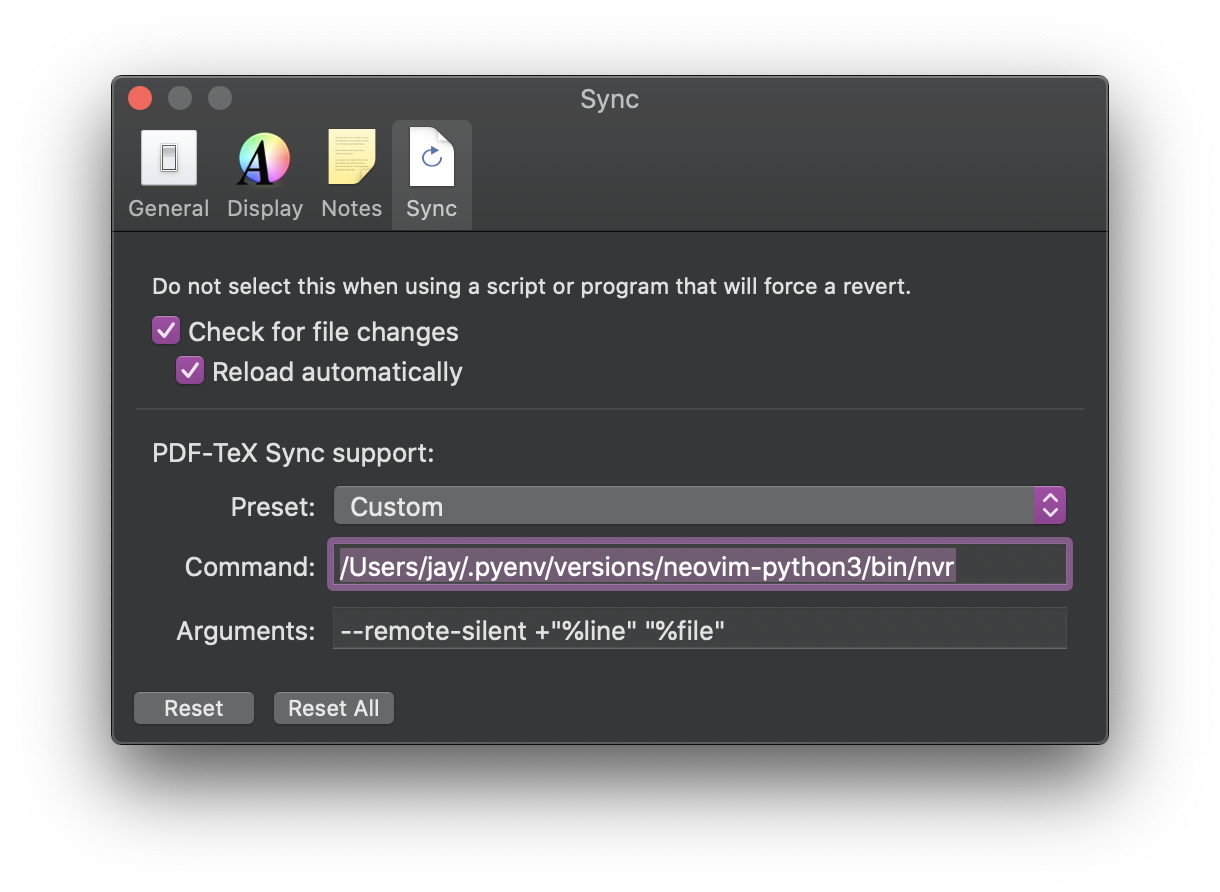
\includegraphics[width=0.9\linewidth]{figures/skim-sync}
  \end{enumerate}
\end{frame}

% Windows setup
\begin{frame}[fragile,allowframebreaks]{\TeX{}nical Vim 설정 (for Windows)}
  Windows용 package manager인 \href{https://chocolatey.org/}{Chocolatey} 사용을
  하며, 이하 명령어들은 PowerShell에서 실행합니다.
  \alert{(Windows 설정은 아직 완벽하지 않습니다.)}
  \begin{enumerate}
    \item \url{https://chocolatey.org/install}을 참고하여
      \href{https://chocolatey.org/}{Chocolatey}를 설치합니다. (명령어가 너무
      길어 링크로 대체)
    \item \href{http://wiki.ktug.org/wiki/wiki.php}{KTUG Wiki}를 참고하여,
      \href{http://mirror.navercorp.com/CTAN/systems/texlive/tlnet/install-tl.zip}{install-tl.zip}의
      압축을 풀고 \textct{install-tl-windows.bat}을 실행하여 설치합니다.
    \item Terminal, SumatraPDF, 그리고 Neovim을 설치합니다.
      \begin{shellcode}
        choco install microsoft-windows-terminal sumatrapdf neovim 
      \end{shellcode}
      \begin{description}
        \item[Windows Terminal] Color scheme (that supports iTerm themes!),
          \alert{option key mapping}, powerline glyphs, ...
        \item[SumatraPDF] Sync\TeX{} support, automatic refresh, ...
      \end{description}

    \framebreak
    \item Python을 설치합니다.
      \begin{itemize}
        \item Python 가상 환경은 Windows용으로
          \href{https://github.com/pyenv-win/pyenv-win}{pyenv-win}이라는 것이
          있다고 합니다.
      \end{itemize}
      \begin{shellcode}
        choco install python3
      \end{shellcode}

    \item \href{https://github.com/mhinz/neovim-remote}{neovim-remote}(nvr)을
      설치합니다.
      \begin{shellcode}
        pip3 install neovim-remote
      \end{shellcode}
      \begin{itemize}
        \item 이는 Skim과 같은 외부 프로그램이 Neovim을 원격으로 조작하여
          reverse search를 가능하게 합니다.
      \end{itemize}

    \framebreak
  \item \url{https://github.com/junegunn/vim-plug#windows-powershell-1}을
    참고하여 Vim plugin manager \href{https://github.com/junegunn/vim-plug}{vim-plug}를 설치합니다.
    \item (Vim을 아신다면) \textct{\tat/AppData/Local/nvim/init.vim}에 다음과
      같이 작성합니다:
      \begin{vimcode}
        call plug#begin('~/AppData/Local/nvim/plugged')
        Plug 'lervag/vimtex'
        call plug#end()
      \end{vimcode}
      그 후 (다시 source하거나) 파일을 다시 열어서 \verb/:PlugInstall/합니다.


    \framebreak
    \item \url{https://github.com/lervag/vimtex/issues/1585} 참고
  \end{enumerate}
\end{frame}

\section{Hello, Vim!}

\begin{frame}[plain]{}
  \begin{columns}
    \begin{column}{0.5\textwidth}
      \centering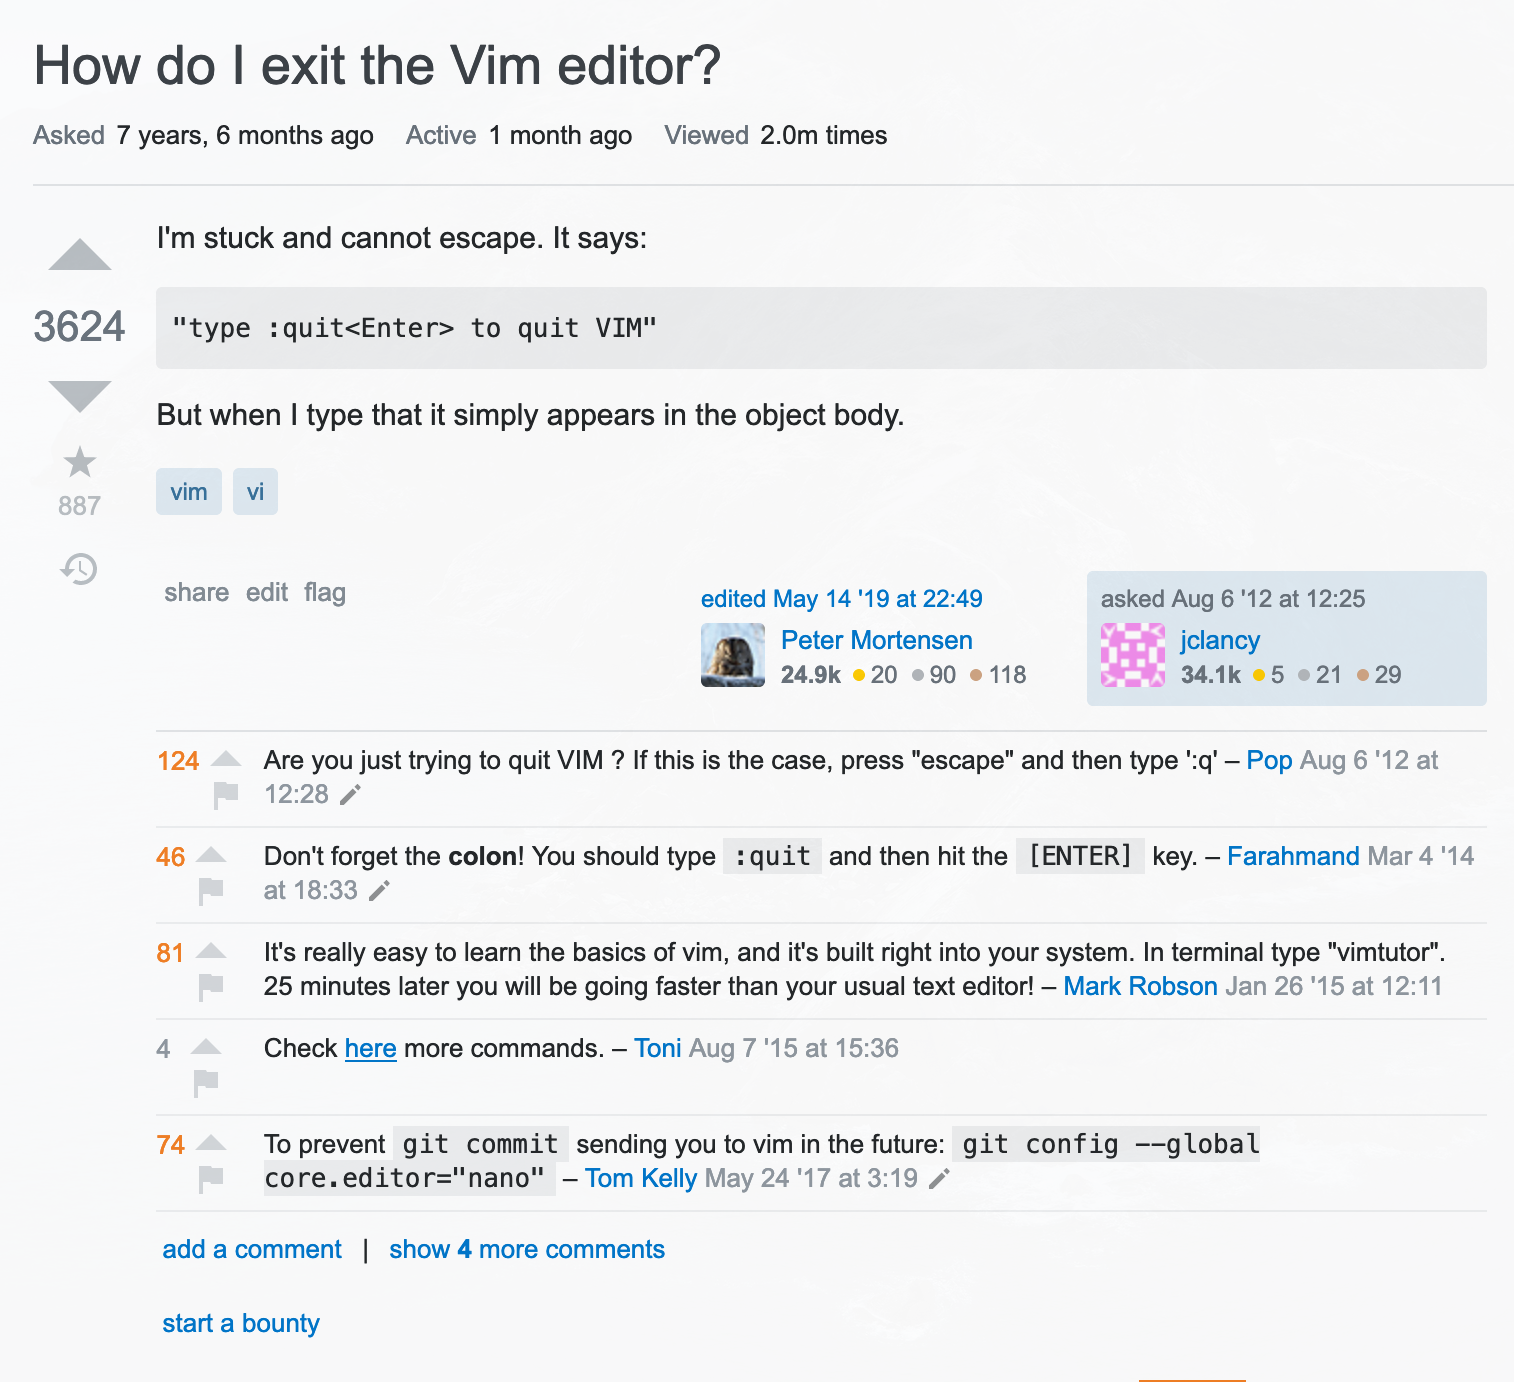
\includegraphics[width=\linewidth]{figures/how-do-i-exit-vim}
    \end{column}
    \begin{column}{0.5\textwidth}
      \centering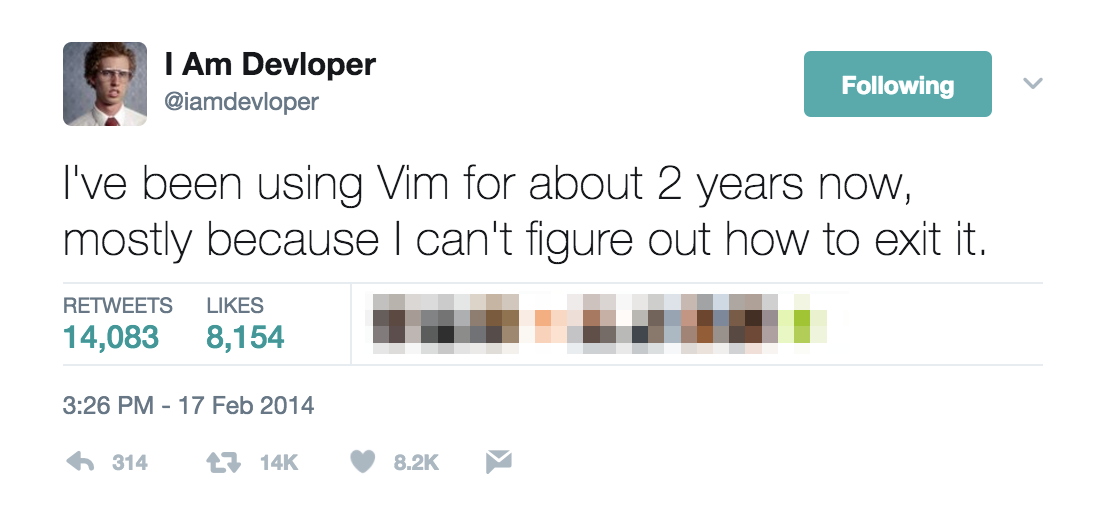
\includegraphics[width=\linewidth]{figures/vim-exit-meme}
    \end{column}
  \end{columns}
\end{frame}

\begin{frame}[fragile]{Exit Vim}
  <Esc>를 두어번 누른 후 (normal 모드로 확실하게 가기),\pause
  \begin{itemize}
    \item \verb/:q/를 친다. (저장 안 된 내용 있을시 오류)\pause
    \item \verb/:q!/를 친다. (저장 안 된 내용 있을시 버리기)\pause
    \item \verb/:wq/를 친다. (저장하고 종료)\pause
    \item \verb/:wq!/를 친다. (읽기 전용이더라도 저장하고 종료)\pause
    \item \verb/:x/를 친다. (저장 안 된 내용 있을시 저장하고 종료)\pause
  \end{itemize}
  이 때 \verb/q/는 \alert{q}uit, \verb/w/는 \alert{w}rite, \verb/x/는
  e\alert{x}it의 약자입니다.\pause
  혹은 normal 모드에서 \verb/ZZ/를 눌러 저장하고 종료하거나 \verb/ZQ/를 눌러
  변경 사항을 버리고 종료할 수 있습니다.
\end{frame}

\begin{frame}[fragile]{The Normal, the Insert, and the Command-line}
  Vim에는 크게 normal, insert, 그리고 command-line 모드가 있습니다.
  (Normal 모드를 command 모드, command-line 모드를 ex 모드라고도 부릅니다.)

  \pause
  모드가 분리되어 있다는 것의 의미:
  \begin{itemize}
    \item GUI 텍스트 에디터에서는 글을 쓰다가, 마우스로 드래그 하다가,
      메뉴바에서 작업을 고르고 하는 일 \pause\tra\, 키보드 위에서 모드를
      바꿔가며 모든 작업을 하는 것
    \item Normal 모드에서는 글을 쓰려고 해도 안 써진다? \pause\tra\, Normal
      모드에서는 cmd, ctrl, alt, fn 등의 불필요한 조합을 (거의) 하지 않고
      명령어를 입력\pause
    \item 작성(insert), 수정(normal), 작업(command-line)을 분리
  \end{itemize}
\end{frame}

\begin{frame}[fragile]{hjkl == \tla\tda\tua\tra}
  Insert 모드에서는 방향키로 이동하지 않습니다.\pause

  Normal 모드에서는 방향키로 이동하지 않습니다.\pause

  Normal 모드에서는 hjkl로 좌하상우로 이동할 수 있습니다.\pause

  \emph{Insert 모드에서는 이동하지 않습니다.}\pause

  \alert{\centering\large Vim에서 모든 일은 normal 모드에서 이뤄집니다.}\pause

  문서에서 이동하거나 작업을 할 때에는 insert 모드에서 <Esc>를 눌러 나온 후,
  normal 모드 혹은 command-line 모드에서 작업해야 합니다.
\end{frame}

\begin{frame}[fragile]{글쓰기}
  Normal 모드에서 insert 모드로 들어가는 방법은 많이 있지만, 다음이 가장
  많이 쓰입니다:
  \begin{itemize}
    \item \verb/i/ - 현재 커서 위치에서 insert 모드로\pause
    \item \verb/a/ - 다음 커서 위치에서 insert 모드로\pause
    \item \verb/I/ - 공백이 아닌 현재 줄의 시작에서 insert 모드로\pause
    \item \verb/A/ - 현재 줄의 끝에서 insert 모드로\pause
    \item \verb/o/ - 새로운 아랫줄에 insert 모드로
    \item \verb/O/ - 새로운 윗줄에 insert 모드로\pause
  \end{itemize}

  \verb/iI/, \verb/aA/, \verb/oO/는 각각 \alert{i}nput, \alert{a}ppend,
  \alert{open}의 약자입니다.
\end{frame}

\begin{frame}[fragile]{글에서 이동하기}
  Normal 모드에서 \verb/hjkl/만으로 이동하는 것은 마치 `1단' 기어와 같아서,
  이것만으로 글을 이동하려면 곤란합니다.
  \begin{columns}
    \begin{column}{0.6\linewidth}
      \begin{itemize}
        \item \verb/w/ - 다음 단어 시작으로\pause
        \item \verb/b/ - 이전 단어 시작으로\pause
        \item \verb/W/ - 공백 기준 다음 단어 시작으로
        \item \verb/B/ - 공백 기준 이전 단어 시작으로\pause
        \item \verb/e/ - 다음 단어 끝으로
        \item \verb/ge/ - 이전 단어 끝으로
      \end{itemize}
    \end{column}
    \begin{column}{0.6\linewidth}
      \begin{itemize}
        \item \verb/E/ - 공백 기준 다음 단어 끝으로
        \item \verb/gE/ - 공백 기준 이전 단어 끝으로\pause
        \item \verb/^/ - 공백이 아닌 현재 줄의 시작으로
        \item \verb/0/ - 현재 줄의 시작으로
        \item \verb/$/ - 현재 줄의 끝으로
        \item \verb/gg/ - 문서 시작으로\pause
        \item \verb/G/ - 문서 끝으로\pause
      \end{itemize}
    \end{column}
  \end{columns}
  \verb/wW/, \verb/bB/, \verb/eE/, \verb/gG/는 각각 \alert{w}ord, \alert{b}ack,
  \alert{e}nd, \alert{g}oto의 약자입니다.
  {\color{gray}\verb|^|와 \verb/$/는 regex의 그것에서 따온 것 같습니다.}
\end{frame}

\begin{frame}[fragile]{count * (operator + motion)}
  위에서 보았던 \verb/w/, \verb/e/ 등은 motion이라고 부릅니다.
  이는 operator와 결합되어 작용합니다:
  \begin{itemize}
    \item \verb/c/ - 수정 (\alert{c}hange)\pause
    \item \verb/d/ - 삭제 (\alert{d}elete)\pause
    \item \verb/y/ - 복사 (\alert{y}ank)\pause
    \item \verb|g~| - 대소문자 바꾸기\pause
    \item \verb/gu/ - 소문자 바꾸기\pause
    \item \verb/gU/ - 대문자 바꾸기 (\alert{U}ppercase)
  \end{itemize}\pause
  예를 들어, \verb/d/(삭제)와 \verb/$/(줄 끝으로)을 같이 써서 \verb/d$/를 쓰면
  줄 끝까지 지우고, 여기에 \verb/5/를 앞에 붙여서 \verb/5d$/를 쓰면 이를 5회
  반복합니다.
\end{frame}

\begin{frame}[fragile]{Text Object}
  마지막으로, \alert{text object}에 대해서 살펴봅시다.
  \verb/apple/이라는 단어에서 커서가 \verb/l/에 있었고, 해당 단어를 지우려면
  지금까지 살펴본 것으로는 \pause\verb/a/로 가기 위해 \verb/b/, 그리고 단어를
  지우기 위해 \verb/dw/를 해야 했습니다.\pause

  그러나 단어 `안', 나아가 어떤 범위에서 편집을 쉽게 하기 위해서 Vim은 text
  object를 제공합니다.

  구조는 \verb/a/ 혹은 \verb/i/와, \verb/"/, \verb/'/, \verb/(/, \verb/)/,
  \verb/w/, \verb/W/ 등을 결합한 것입니다.\pause

  예를 들어, \verb/iw/은 `단어 안', \verb/aw/은 `(띄어쓰기를 포함한)
  단어'입니다.
  각각 ``inner word'', ``a word''라고 읽으시면 됩니다.\pause

  따라서, 이를 operator와 결합하여 \verb/cis/와 같이 쓸 수 있습니다.
\end{frame}

\begin{frame}{더 읽을거리}
  \begin{itemize}
    \item \href{https://neovim.io/}{neovim.io}
    \item \href{https://vimawesome.com/}{Vim Awesome}
    \item \href{http://www.viemu.com/a-why-vi-vim.html}{Why, oh WHY, do those \#?\@! nutheads use vi?}
    \item \href{http://vimcasts.org/}{Vimcasts.org}
  \end{itemize}
\end{frame}

\section{\TeX{}nical Vim}

\begin{frame}{Neovim + Vimtex + Coc.nvim + TexLab = $\heartsuit$}
  \begin{description}
    \item[\href{https://neovim.io/}{Neovim}] 모던 Vim (The Engine)
    \item[\href{https://github.com/lervag/vimtex}{Vimtex}] \TeX{} 문서를
      Vim에서 쉽게 쓸 수 있도록 motion, text objects, 기타 mapping을 제공하며,
      문서 navigation, PDF 뷰어들과의 연동을 담당
    \item[\href{https://github.com/neoclide/coc.nvim}{Coc.nvim}] Vim 8/Neovim을
      위한 IntelliSense engine입니다. LSP를 지원하며, 나아가 VS Code용 plugin을
      Vim에서 쓸 수 있게 합니다.
    \item[\href{https://texlab.netlify.com/}{TexLab}] Crossplatform \LaTeX{} /
      Bib\TeX{} language server입니다.
  \end{description}
\end{frame}

\begin{frame}{Language Server Protocol (LSP)란?}
  \centering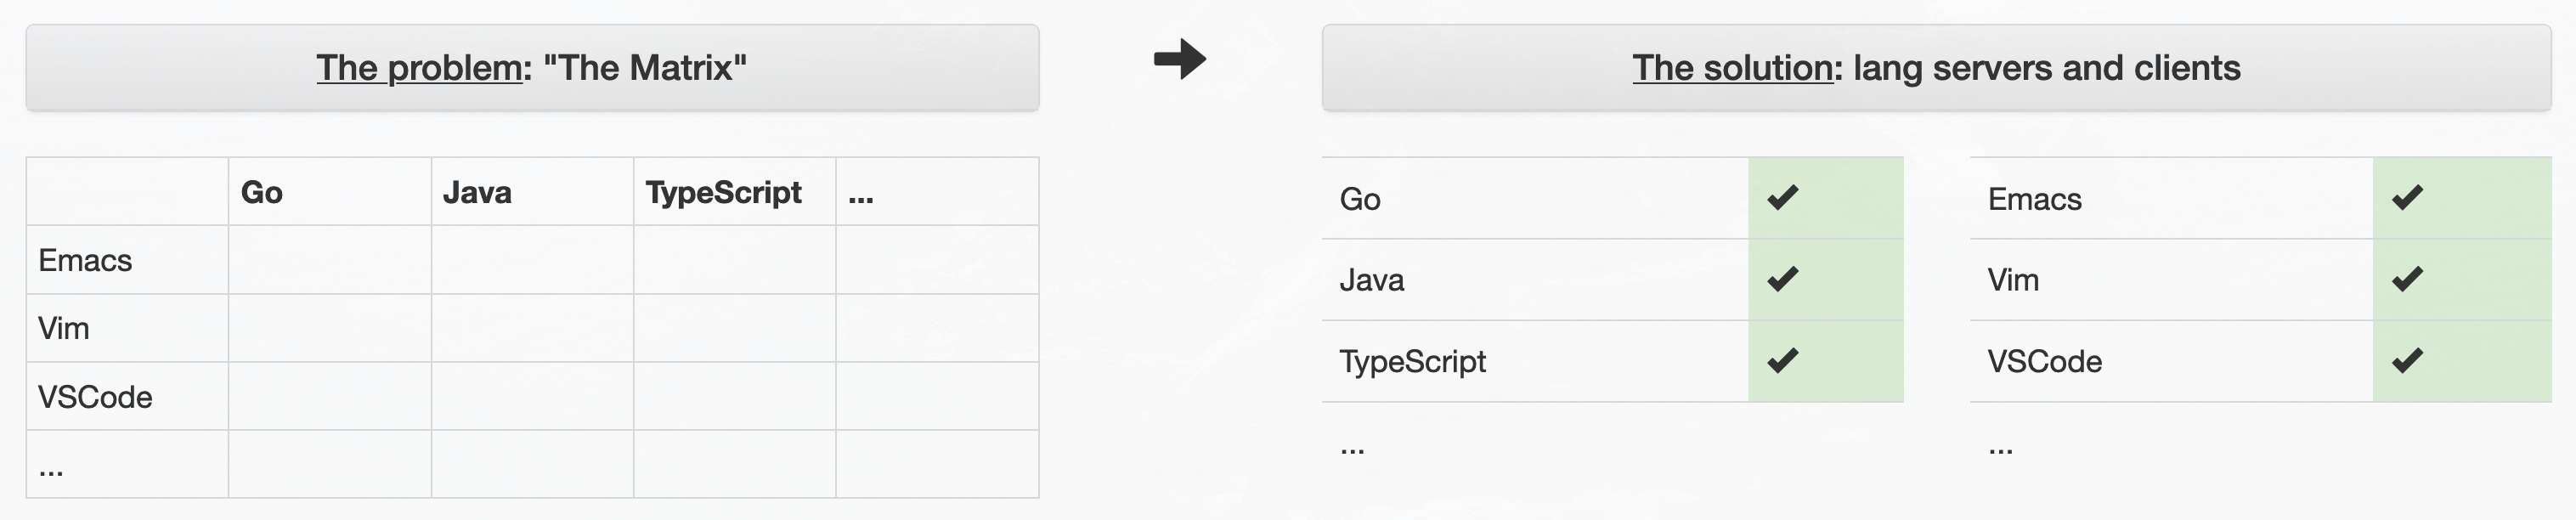
\includegraphics[width=\linewidth]{figures/lsp-solution}
  {\tiny 출처: \url{https://langserver.org/}}

  자동 완성, 문법 강조, 문서 등의 언어 분석 기능을 가진 language server와 IDE
  및 에디터 (client) 간의 규약으로, Microsoft가 VS Code를 만들면서
  공개하였습니다.
\end{frame}

\begin{frame}[fragile]{Last Vim Setup}
  TexLab은 macOS의 경우 \textct{brew install texlab}으로, Windows의 경우
  \url{https://github.com/latex-lsp/texlab/releases}에서 설치할 수 있습니다.

  Vimtex과 coc.nvim은 vim-plug로 설치하면 되는데, \textct{init.vim}에 아래와
  같이 추가하면 됩니다:
  \begin{vimcode}
    call plug#begin('~/.local/share/nvim/plugged')
    Plug 'lervag/vimtex'
    Plug 'neoclide/coc.nvim', { 'branch': 'release' }
    call plug#end()
    let g:vimtex_view_method = 'skim'
    let g:coc_global_extensions = ['coc-texlab']
  \end{vimcode}

  Neovim을 껐다 켠 후 \textct{:PlugInstall} 해줍니다.
  이외 coc.nvim의 예시 설정: \url{https://github.com/neoclide/coc.nvim}
\end{frame}

\begin{frame}[fragile]{\texttt{init.vim} / \texttt{.vimrc}}
  지금까지는 Vim을 조작하는 방법에 대해서 알아보았는데요, 지금은 간단히 Vim의
  설정을 바꾸어 그냥 `검은 화면'을 바꾸어 봅시다.

  \pause
  이런 설정은 Vim을 실행하여 command-line mode에서 \textct{:set nu} 등과 같이
  바꿀 수 있습니다.
  그런데 이를 매번 실행할 수는 없으므로, 매번 Vim이 확인해서 실행하는 파일이
  바로 Vim의 \textct{.vimrc} 혹은 Neovim의 \textct{init.vim} (XDG 기반)입니다.

  \pause
  \textct{call plug\#end()} 밑에 아래와 같이 추가하면 Vim 옆에 상대적인 줄번호와
  색상이 추가된 것을 볼 수 있습니다:
  \begin{vimcode}
    set number
    set relativenumber
    colorscheme slate
  \end{vimcode}
\end{frame}

\begin{frame}[fragile]{자동 완성, 추가된 Text Objects}
  Vimtex과 TexLab 모두 자동 완성 기능을 제공하며, 각 추천어들은 <C-n>과 <C-p>로
  선택할 수 있으며 <CR> (return)키를 통해 snippet을 확장할 수도 있습니다.

  \pause
  Text object의 경우 Vimtex이 제공하는데, command나 환경을 쉽게 바꾸고
  \verb|*|를 넣거나 빼기가 굉장히 편합니다.
  예를 들어서 \verb/tsc/ (``toggle surrounding command'')는 명령어에 \verb|*|를
  넣고 빼주며, \verb/dae/ (``delete an environment'')는 현재 환경
  \textct{\tbs begin\{env\}...\tbs end\{env\}}을 지웁니다.
\end{frame}

\begin{frame}[fragile]{편한 Mappings}
  \begin{itemize}
    \item \verb/\ll/ - 연속 조판 (저장할 때마다 조판하기)
    \item \verb/\lv/ - Forward search
    \item \verb/\le/ - 조판 오류 보기
    \item \verb/\lc/ - 부수 파일 삭제
    \item \verb/\lC/ - 부수 파일 및 PDF 삭제
    \item \verb/\lt/ - 문서 목차 보기
    \item \verb/\lt/ - 문서 목차 toggle
    \item \verb/K/ - \verb/texdoc/ 없이 package의 개요 보기
  \end{itemize}
\end{frame}

\begin{frame}[fragile]{Forward / Backward Search (Sync\TeX)}
  \begin{center}
    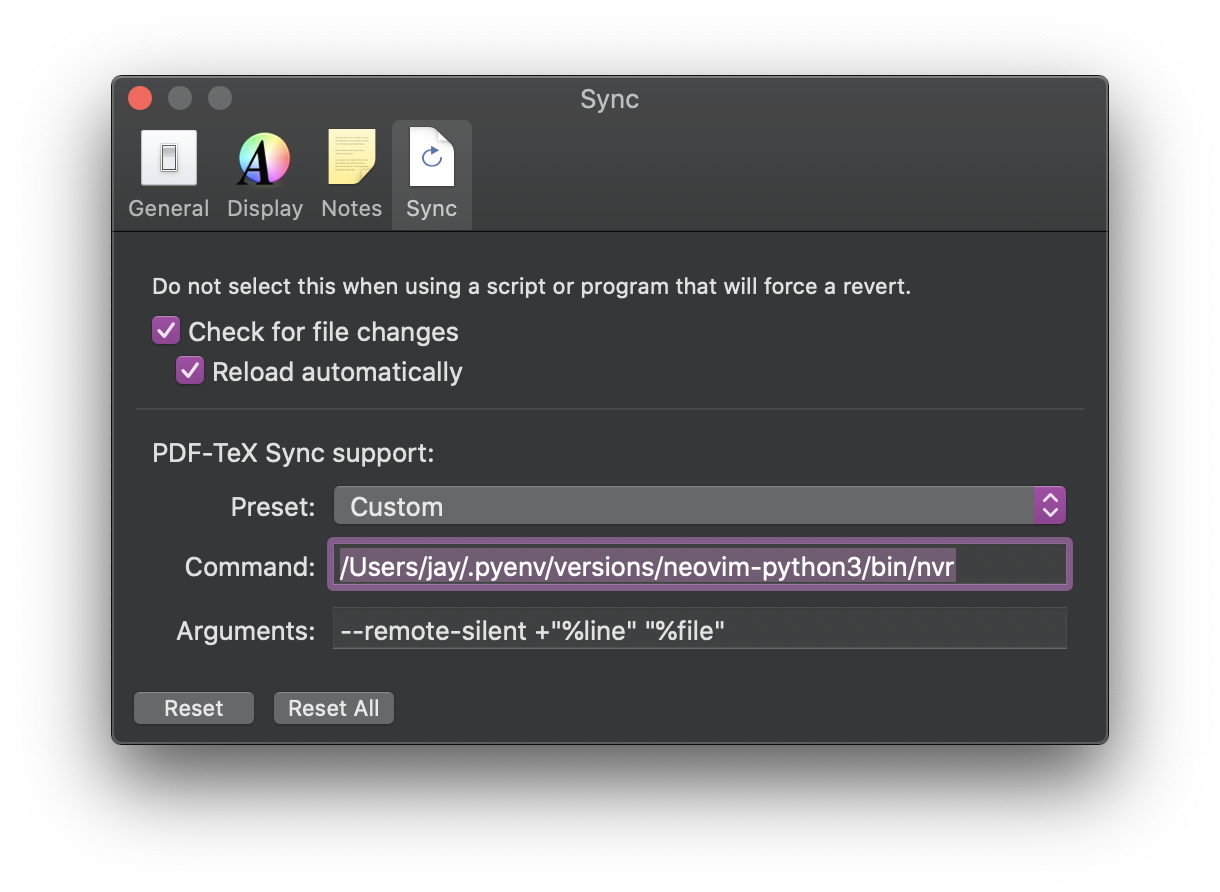
\includegraphics[width=0.6\linewidth]{figures/skim-sync}
  \end{center}

  Neovim은 \textct{NVIM\_LISTEN\_ADDRESS=/tmp/nvimsocket nvim}로 시작하면
  됩니다.
  매번 칠 수 없으므로 alias를 만듭니다:
  \begin{shellcode}
    alias v='NVIM_LISTEN_ADDRESS=/tmp/nvimsocket nvim'
  \end{shellcode}
\end{frame}

\begin{frame}{P.S. Neovim에 버그가 있는 것 같아요...}
  \centering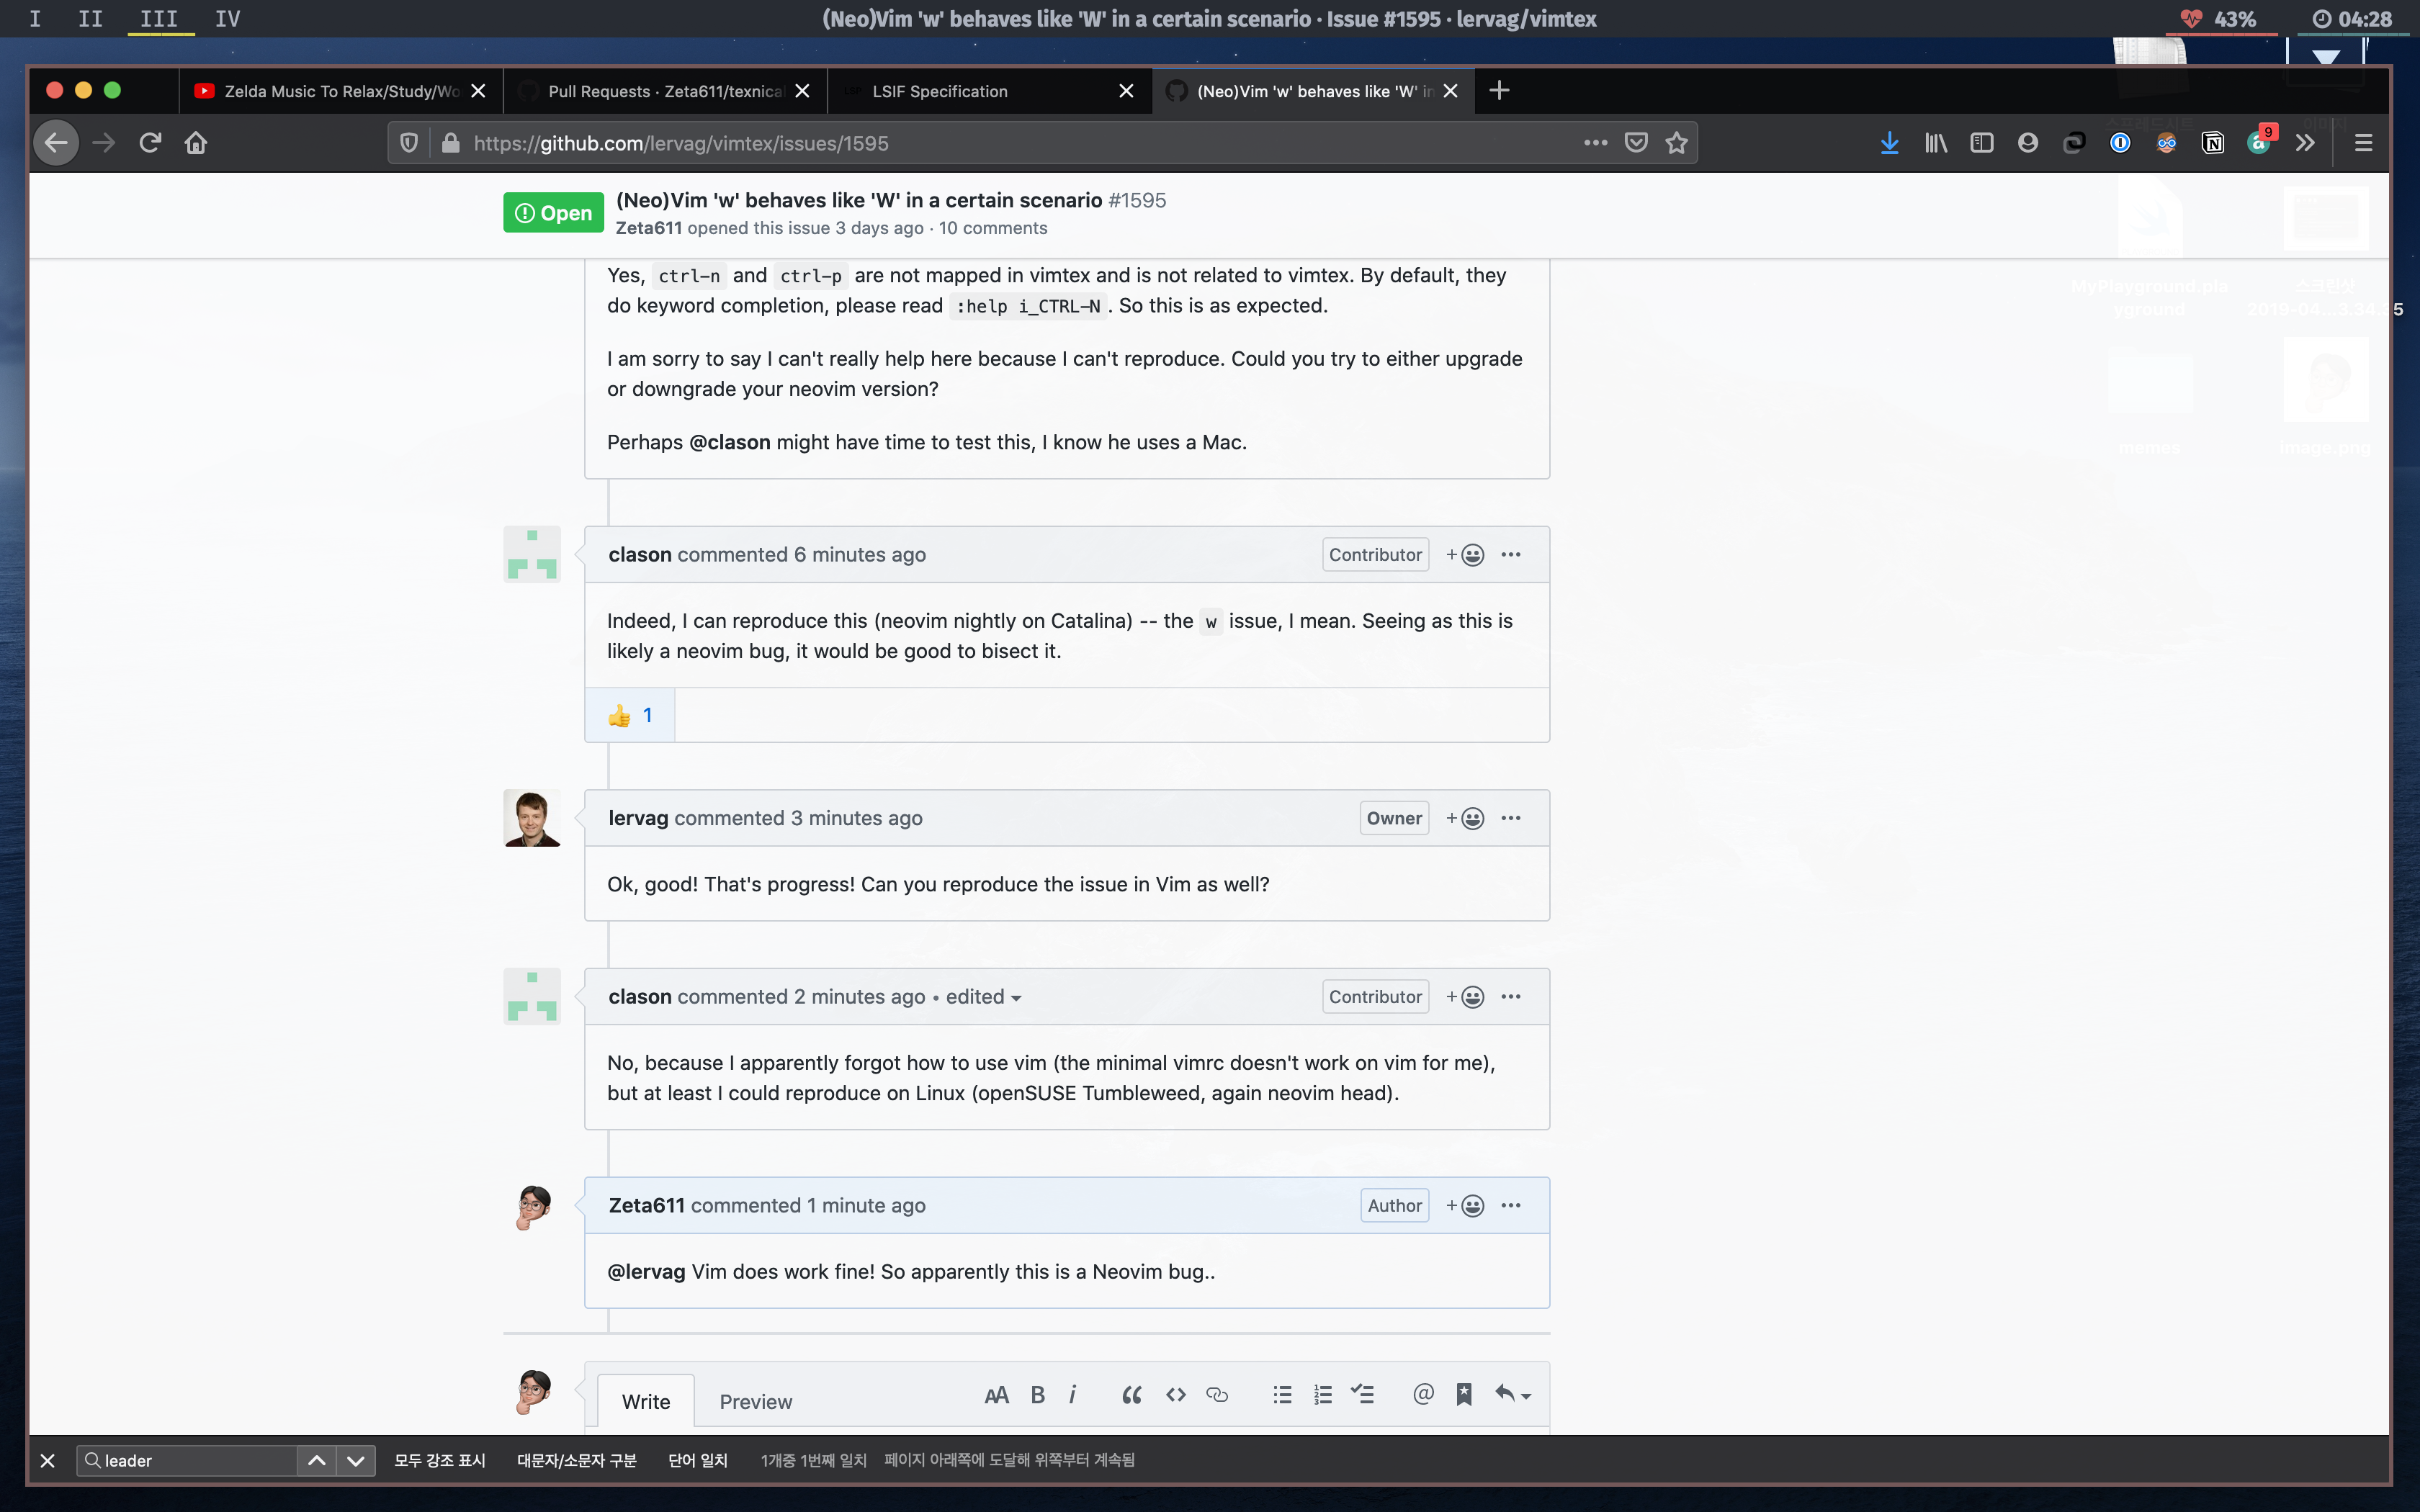
\includegraphics[width=\linewidth]{figures/neovim-issue}
  \url{https://github.com/lervag/vimtex/issues/1595}
\end{frame}

\begin{frame}[standout]
  감사합니다.
\end{frame}

\begin{frame}{부록}
  발표 자료: \url{https://github.com/Zeta611/texnical-vim-kts-conf-2020}

  Neovim 설정: \url{https://github.com/Zeta611/dotfiles}

  \centering
\includegraphics[width=0.35\linewidth]{figures/how-great-vim-is}
\end{frame}

\section{\texorpdfstring{$+\alpha$}{+⍺}}
\begin{frame}{추가 자료}
  발표가 끝난 후, `어떤 자료가 있으면 좋을 것 같다'는 의견이 있어서 자료를
  추가합니다.
  내용을 중간에 보충하려다가 업데이트된 부분을 쉽게 보실 수 있도록 뒤에
  추가하여 정리합니다.
\end{frame}

\begin{frame}[allowframebreaks,fragile]{1. 자동 한/영 전환}
  Vim에서 한글 \TeX{} 문서를 작성하신다면, normal 모드의 명령어를 영어로
  입력하다가 insert 모드에서 한글로 입력을 하기 위해 한/영 전환을 하는 것이
  상당히 불편합니다.

  이를 위해서 (macOS에서)
  \href{https://github.com/vovkasm/input-source-switcher}{input-source-switcher}와
  Vim plugin인 \href{https://github.com/lyokha/vim-xkbswitch}{vim-xkbswitch}을
  사용합니다.

  \framebreak
  다음과 같이 input-source-switcher을 설치합니다.
  cmake에 \verb/-DCMAKE_INSTALL_PREFIX:PATH=$HOME/을 준 이유는 홈 디렉터리에
  설치하기 위함입니다.
  옵션을 안 주면 기본 설치 경로에 설치됩니다.
  터미널에서 다음과 같이 실행합니다:
  \begin{shellcode}
    git clone https://github.com/vovkasm/input-source-switcher.git
    cd input-source-switcher
    mkdir build && cd build
    cmake -DCMAKE_INSTALL_PREFIX:PATH=$HOME ..
    make
    make install
    cd ../..
  \end{shellcode}

  \framebreak
  이제 Vim에서 vim-xkbswitch를 설정하면 됩니다.
  \verb/init.vim/에 다음과 같이 추가합니다:
  \begin{vimcode}
    call plug#begin('~/.local/share/nvim/plugged')
    Plug 'lyokha/vim-xkbswitch'
    call plug#end()

    let g:XkbSwitchEnabled = 1
    let g:XkbSwitchLib = expand('~/lib/libInputSourceSwitcher.dylib')
    " 기본 경로에 설치했다면 아래와 같이 설정합니다:
    " let g:XkbSwitchLib = '/usr/local/lib/libInputSourceSwitcher.dylib'
  \end{vimcode}
\end{frame}
\end{document}
